%  section on run scenarios

% CHAPTER ON ILC RUNNING SCENARIOS

One of the key advantages of $e^+e^-$ colliders is the ability to collect individual datasets at at a series of different center-of-mass energies and beam polarisation settings.   While each measurement one might wish to make has its own prefered data-taking mode, the combination with datasets collected at other beam energies and/or beam polarisations provides a unique robustness against systematic uncertainties.  This is obvious for data-taking at different energies, but it is also
true for data-taking at different polarizations. For example, a recent PhD thesis~\cite{Habermehl:417605} studied Dark Matter searches with consideration of  non-neglibigle systematic uncertainties and showed that one obtains better results by  sharing a given amount of total integrated luminosity between datasets with different beam polarisations rather than by investing the same total amount of luminosity into the (statistically) most favourable polarisation configuration.

Any physics projection will therefore depend on the exact running scenario, i.e.\ the ensemble of the integrated luminosities collected at the individual center-of-mass energies with the various polarisation settings. For the physics conclusions given in this paper, we have assumed the energy and luminosity evolution of the ILC shown 
in Fig.~\ref{fig:H20staged}.  At each energy, the time is shared among the various choices for beam polarization in the manner explained in Sec.~\ref{subsec:runscen_pol}.
The full physics program is projected to take 22 years, including a realistic learning 
curve for the establishment of luminosity and scheduled downtimes for luminosity and energy upgrades.   In this schedule, the ILC would accumulate 2\,ab$^{-1}$ at 250\,GeV by year 11.  It woud then add datasets of 0.2\,ab$^{-1}$ at 350\,GeV and  4\,ab$^{-1}$ at 500\,GeV by year 22. 

%%%%%%%%%%%%%%%%%%%%%%%%%%%%%%%%%%%%%%%%%%%%%%%%%%%%%%%%%%%%%%%%%%%%%%%%%
\begin{figure}
\begin{center}
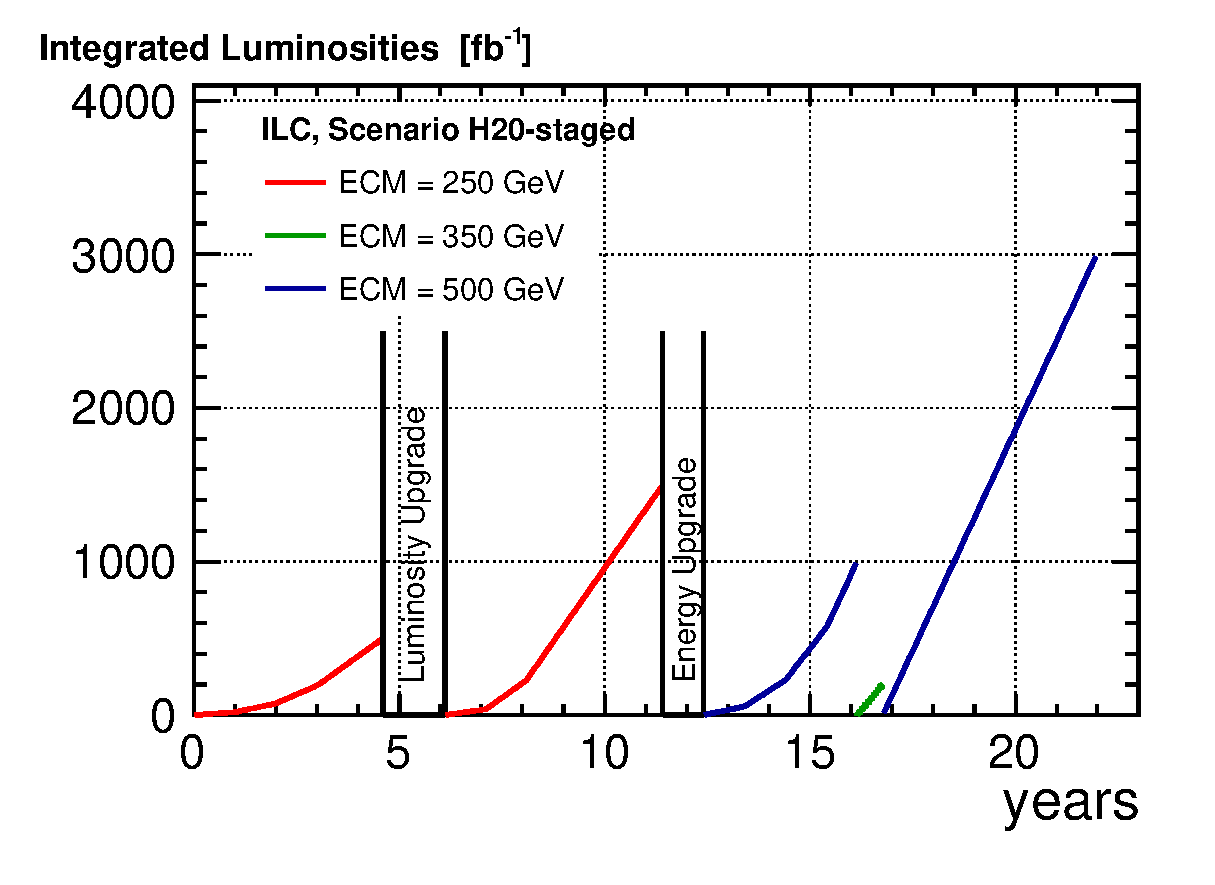
\includegraphics[width=0.90\hsize]{chapters/figures/lumi_H20-staged}
\end{center}
\caption{The nominal 22-year running program for the staged ILC, starting operation at 250\,\GeV with the current baseline beam parameters for the 250\,GeV runs~\cite{Fujii:2017vwa}. }
\label{fig:H20staged}
\end{figure}
%%%%%%%%%%%%%%%%%%%%%%%%%%%%%%%%%%%%%%%%%%%%%%%%%%%%%%%%%%%%%%%%%%%%%%%%%%%


The interplay between different datasets has been studied in detail in~\cite{Barklow:2015tja}, with a special focus on the optimisation of the Higgs precision measurements, resulting in a standard running scenario for ILC physics projections. The time evolution of this running scenario has been adapted to the staged construction of the ILC as first presented in~\cite{Fujii:2017vwa}. 

In this section, we will discuss the considerations that have entered the choice of this running scenario, the evolution of this scenario in accord with the design of the 
ILC accelerator, and the flexibility of the plan to respond to changes in machine
specifications or physics discoveries.

\subsection{Center-of-mass energies and integrated luminosities}
The three center-of-mass energies for ILC best motivated by our current knowledge are:
\begin{itemize}
\item $\sqrt{s}=250$\,GeV for collecting data near the threshold of the Higgsstrahlungs process, 
\item $\sqrt{s}=350$\,GeV for scanning the threshold for top quark pair production, and 
\item $\sqrt{s}=500$\,GeV or somewhat above for studying $t\bar{t}$ production in the continuum and enabling $t\bar{t}H$ and $ZHH$ production. 
\end{itemize}
Table~\ref{tab:lumiabstot} gives the total integrated luminosities foreseen at these energies for three alternative running scenarios.  These scenarios are described in~\cite{Barklow:2015tja},  which presented a detailed evaluation of these and other possibilities.  For comparison,  the integrated luminosities assumed in the Snowmass community study~\cite{Asner:2013psa}  is given in the last column. Since 2015, the scenario H20 has been  the reference scenario for ILC physics projections.

\begin{table}[h]
\centering
  \renewcommand{\arraystretch}{1.10}
\begin{tabularx}{\columnwidth}{*{4}{>{\centering\arraybackslash}X} || *{1}{>{\centering\arraybackslash}X}} 
%\begin{tabular*}{\textwidth}{@{\extracolsep{\fill}}c|c c c c c}
%\begin{tabular}{|l||c|c|c|c|c|}
\hline
            &  \multicolumn{4}{c}{$\int{\mathcal{L} dt}$ [fb$^{-1}$]} \\
\hline
$\sqrt{s}$  & G20      &   H20   &  I20   & Snow   \\
\hline
250\,GeV    &  500      &  2000    &   500   & 1150   \\
350\,GeV    &  200      &   200    &  1700   &  200  \\
500\,GeV    & 5000      &  4000    &  4000   & 1600  \\
\hline
%\end{tabular*}
\end{tabularx}
\caption{Proposed total target integrated luminosities for $\sqrt{s}=250$,  $350$, $500$\,GeV based on $20$ ``real-time'' years of ILC operation under scenarios G20, H20 and I20. The total integrated luminosities assumed for Snowmass
are listed for comparison based on 13.7 ``real-time'' years. From~\cite{Barklow:2015tja}.}
\label{tab:lumiabstot} 
\end{table}


It must be stressed, however, that flexibility in the run plan remains one of the key assets of the ILC.  This plan can be adjusted whenever new insights,  discoveries either from the (HL-)LHC or from the ILC itself, require us to do so. In particular, the center-of-mass energy of the ILC can always be lowered from the nominal maximum energy without loss of efficiency and/or luminosity, as long as the electron beam energy remains sufficiently high for positron production. In fact, the operation of the SCRF cavities below the maximum gradient
saves significant cryogenic and RF power, which in turn can be invested into higher instantaneous luminosity.

Future $e^+e^-$ colliders could also provide important physics measurements at other center-of-mass energies. Physics goals that motivate other choices are the high-statistics study of $Z$ and $W$, the exploration of the thresholds for any new color-singlet particles that might appear in the ILC energy region, and data-taking at additional center of mass energies to optimize the determination of Effective Field Theory parameters. The lower center-of-mass energies could be realized by doubling the repetition rate of the electron linac to 10\,Hz and adding a by-pass around the positron source for every second bunch train. Today, however, the priority of these issues seems lower than that  for the abovementioned three energies. Therefore they are not explicitly included in the current run plan of the ILC or in the current set of machine parameters.  Over a longer term, we plan to extend the linac to reach 
energies of 1\,TeV or higher.   Table~\ref{tab:lumiabstot1TeV} lists target integrated luminosities approriate to physics studies at these additional energies.

\begin{table}[h]
\centering
  \renewcommand{\arraystretch}{1.10}
\begin{tabularx}{\columnwidth}{l *{4}{>{\centering\arraybackslash}X}} 
%\begin{tabular*}{\textwidth}{@{\extracolsep{\fill}}c|c c c c c}
%\begin{tabular}{|l||c|c|c|c|c|}
\hline
$\sqrt{s}$     &  90\,GeV & 160\,GeV  &    1\,TeV \\
\hline
 $\int{\mathcal{L} dt}$ [fb$^{-1}$]         	   &  100       &  500    & 8000 \\
\hline
%\end{tabular*}
\end{tabularx}
\caption{Proposed total target integrated luminosities for other $\sqrt{s}$.  From~\cite{Barklow:2015tja}.}
\label{tab:lumiabstot1TeV} 
\end{table}


\subsection{Beam polarisation}
\label{subsec:runscen_pol}
At center-of-mass energies of up to 500\,GeV, the ILC beams are foreseen to be polarised  with absolute values of at least 80\% for the electrons and at least 30\% for the positrons. At 1\,TeV, the positron polarisation will reach at least 20\%. As an upgrade option, the positron polarisation can be increased to 60\% for center-of-mass energies around 500\,GeV; this is discussed in Sec.~\ref{subsubsec:upg-optP}. The accelerator design comprises sets of spin rotators which in principle allow one to prepare any desired direction of the polarisation vectors at the IP. However in the detailed running scenarios, we consider only longitudinal polarisation. The sign of the beam polarisations can be flipped 
on a train-by-train basis. This allows us to collect datasets with different helicity configurations quasi-concurrently compared to the typical time scales of changes in the accelerator or detector configuration, calibration and alignment. In a joint analysis of these datasets, large parts of the experimental systematic uncertainties cancel.  This is particularly important to minimize the 
systematic errors in the measurement of the left-right polarization asymmetry, a quantity that carries a great deal of information for every process that will be studied at the ILC.  But this idea has many other applications. The joint interpretation of the different datasets allows us to treat many systematic effects as nuisance parameters in global fits, and thereby to measure and subtract these effects~\cite{bib:PhDRobert}. 

The role of positron polarisation specifically at an initial 250-GeV stage of the ILC has been discussed in detail in a recent document~\cite{Fujii:2018mli}. In the case of a global fit to polarised total and differential cross-sections of various electroweak processes, it is shown there  that the uncertainties on some observables increase by up to a factor of 10 in the absence of positron polarisation due to the lack of redundancies required for ultimate control of systematic uncertainties. As we will see in Sec.~\ref{subsec:phys_eft}, the left-right asymmetry $A_{LR}(HZ)$ of the Higgsstrahlungs cross section plays an important role in our technique for obtaining a  model-independent fit to Higgs couplings.  Although the measurement of the absolute normalization of the Higgsstrahlungs cross section was not explicitly included in the study summarized in~\cite{Fujii:2018mli}, analogous deteriorations would also be expected for this quantity.

A part of the power of positron polarisation is that it allows one to collect four independent data sets with different mixtures of the physics reactions under study.   Tables~\ref{tab:pollumirel} through~\ref{tab:pollumiabs1TeV} give our
standard assumptions for the sharing of the total integrated luminosity (c.f.\ Tab.~\ref{tab:lumiabstot} and~\ref{tab:lumiabstot1TeV}) between the four possible beam helicity combinations. Due to the importance of  $A_{LR}(HZ)$~\cite{Durieux:2017rsg, Barklow:2017suo} noted above, the sharing for 250\,GeV, which was originally foreseen~\cite{Barklow:2015tja} to emphasize the $\operatorname{sgn}(P(e^-),P(e^+))=(-,+)$ configuration, is now  adjusted to provide equal amounts of luminosity for $(-,+)$ and $(+,-)$~\cite{Barklow:2017suo, Fujii:2017vwa}.

These integrated luminosities and polarisation configurations, especially as specified in Tab.~\ref{tab:pollumiabs} for the H20 running scenario, define the reference scenario for all ILC physics projections.  The order in which the various energies are surveyed will of course depend on the machine evolution and staging plan.

\begin{table}[h]
\centering
  \renewcommand{\arraystretch}{1.10}
\begin{tabularx}{\columnwidth}{l *{4}{>{\centering\arraybackslash}X}} 
%\begin{tabular*}{\textwidth}{@{\extracolsep{\fill}}|c|c|c|c|c|c|}
%\begin{tabular}{|l||c|c|c|c|c|}
\hline
        & \multicolumn{4}{c}{fraction with $\operatorname{sgn}(P(e^-),P(e^+))= $ } \\
           & (-,+) & (+,-) & (-,-) & (+,+) \\
\hline
$\sqrt{s}$ & [\%]  &  [\%] & [\%]  & [\%]  \\ 
\hline
250\,GeV (2015)   & 67.5 &  22.5 &  5    &   5   \\
250\,GeV (update) & \bf{45} &  \bf{45} &  5    &   5   \\
350\,GeV   & 67.5 &  22.5 &  5    &   5   \\
500\,GeV   &  40  &  40   &  10   &  10   \\
\hline
%\end{tabular*}
\end{tabularx}
\caption{Relative sharing between beam helicity configurations proposed for the various center-of-mass energies. The update of the luminosity
sharing for 250\,GeV originates from the importance of the left-right asymmetry of the Higgsstrahlung cross section in the EFT-based Higgs coupling fit.}
\label{tab:pollumirel} 
\end{table}

\begin{table}[h]
\centering
  \renewcommand{\arraystretch}{1.10}
\begin{tabularx}{\columnwidth}{l *{4}{>{\centering\arraybackslash}X}}    %\begin{tabular*}{\textwidth}{@{\extracolsep{\fill}}|c|c|c|c|c|}
%\begin{tabular}{|l|c|c|c|c|}
\hline
        &  \multicolumn{4}{c}{int. luminosity with $\operatorname{sgn}(P(e^-),P(e^+))= $ } \\
           & (-,+)       & (+,-)       & (-,-)       &  (+,+)     \\
\hline
$\sqrt{s}$ & [fb$^{-1}$] & [fb$^{-1}$] &  [fb$^{-1}$] & [fb$^{-1}$] \\ 
\hline
250\,GeV (2015)   &  1350      &  450        &  100	      &   100  \\
250\,GeV (update) &  \bf{900}  &  \bf{900}   &  100	      &   100  \\
350\,GeV          &   135      &   45	     &   10	      &    10  \\
500\,GeV          &  1600      & 1600        &  400	      &   400  \\
\hline
\end{tabularx}
\caption{Integrated luminosities per beam helicity configuration resulting from the fractions in table~\ref{tab:pollumirel} in scenario H20. The update of the luminosity
sharing for 250\,GeV originates from the importance of the left-right asymmetry of the Higgsstrahlung cross section in the EFT-based Higgs coupling fit. 
}
\label{tab:pollumiabs} 
\end{table}

\begin{table}[h]
\centering
  \renewcommand{\arraystretch}{1.10}
\begin{tabularx}{\columnwidth}{l *{4}{>{\centering\arraybackslash}X}} 
%\begin{tabular*}{\textwidth}{@{\extracolsep{\fill}}|c|c|c|c|c|c|}
%\begin{tabular}{|l||c|c|c|c|c|}
\hline
        & \multicolumn{4}{c}{fraction with $\operatorname{sgn}(P(e^-),P(e^+))= $ } \\
           & (-,+) & (+,-) & (-,-) & (+,+) \\
\hline
$\sqrt{s}$ & [\%]  &  [\%] & [\%]  & [\%]  \\ 
\hline
90\,GeV    &  40  &  40   &  10   &  10   \\
160\,GeV   & 67.5 &  22.5 &  5    &   5   \\
1\,TeV     &  40  &  40   &  10   &  10   \\
\hline
%\end{tabular*}
\end{tabularx}
\caption{Relative sharing between beam helicity configurations proposed for low energy and $1$\,TeV running. From~\cite{Barklow:2015tja}.}
\label{tab:pollumirel1TeV} 
\end{table}

\begin{table}[h]
\centering
  \renewcommand{\arraystretch}{1.10}
\begin{tabularx}{\columnwidth}{l *{4}{>{\centering\arraybackslash}X}}    %\begin{tabular*}{\textwidth}{@{\extracolsep{\fill}}|c|c|c|c|c|}
%\begin{tabular}{|l|c|c|c|c|}
\hline
        &  \multicolumn{4}{c}{integrated luminosity with $\operatorname{sgn}(P(e^-),P(e^+))= $ } \\
           & (-,+)       & (+,-)       & (-,-)       &  (+,+)     \\
\hline
$\sqrt{s}$ & [fb$^{-1}$] & [fb$^{-1}$] &  [fb$^{-1}$] & [fb$^{-1}$] \\ 
\hline
90\,GeV     &    40   	 &   40        &   10	      &    10  \\
160\,GeV    &   340   	 &  110        &   25	      &    25  \\
1\,TeV      &  3200   	 & 3200        &  800	      &   800  \\
\hline
\end{tabularx}
\caption{Integrated luminosities per beam helicity configuration resulting from the fractions in table~\ref{tab:pollumirel1TeV}. From~\cite{Barklow:2015tja}.}
\label{tab:pollumiabs1TeV} 
\end{table}


\subsection{Time Evolution and Upgrade Options}

The possible real-time evolution of the integrated luminosity was studied in detail in~\cite{Barklow:2015tja}.  It is important to note that the plans given in that study assumed that the full 500\,GeV machine would be available from the beginning. With the introduction of a staged construction plan for the ILC, the time ordering of 
different runs needed to be adjusted. However, the details of trade-offs between scenarios is most fully documented in 
\cite{Barklow:2015tja}, so we will first review that study and the logic of its conclusions.   After this, we will describe our
current plan for the run scenario including the constraints from staging. 

\subsubsection{Running Scenarios for the 500-GeV Machine}
\label{subsubsec:runscen_ilc500}

In the study \cite{Barklow:2015tja}, the peak luminosities used for each centre-of-mass energy are based on the numbers published in the ILC TDR~\cite{Adolphsen:2013jya}. But then, the plans took advantage of the reduced linac  electrical power and cryogenic loads when operating the full 500\,GeV machine at lower gradients.  This in particular allows 10-Hz and 7-Hz running, respectively, at the 250\,GeV  and 350\,GeV centre-of-mass energies. In addition, a luminosity upgrade (from 1312 to 2625 bunches per pulse) was been considered; this could require the installation of an additional positron damping ring, as described in  Sec.~\ref{subsubsec:upg-optL}.

More specifically, the study \cite{Barklow:2015tja} made the following assumptions:

\begin{itemize} 
\item A full calendar year is assumed to represent eight months running at an efficiency of 75\% as assumed in the ILC RDR~\cite{Phinney:2007gp}. This corresponds approximately to $Y= 1.6 \times 10^7$ seconds of integrated
running, thus 60\% more than a ``Snowmass year'' of $10^7$ seconds.
\item The start of ``Year 1'' is the start of running for physics. After the end of construction, there is one year foreseen for machine commissioning only, which is not shown on the plots.
\item A ramp-up of luminosity performance, defined as a set of yearly ramp factors $f \le 1$, is in general assumed after: (a) initial construction and `year 0' commissioning; (b) a downtime for a luminosity upgrade; (c) a change in operational mode which may require some learning curve (\eg,  going to 10-Hz collisions).
\item If the peak instantaneous luminosity is $L$, then the nominal integrated luminosity for any given
calendar year is $\int \mathcal{L} dt = f \times L \times Y$, where $f$ is the ramp factor associated with that year.
\item The peak instantaneous luminosities are those corresponding to the TDR beam parameters at 250, 350 and 500\,GeV, as shown in Tab.~\ref{tab:ilc-params}.
\item For the initial physics run after construction and year 0 commissioning, the RDR ramp of 10\%,
30\%, 60\% and 100\% over the first four calendar years is always assumed.
\item  The ramp after the shutdown for installation of the luminosity upgrade is assumed to be slightly shorter (10\%, 50\%, 100\%) with no year 0.
\item Going down in centre of mass energy from $500$\,GeV to $350$\,GeV or $250$\,GeV is assumed to have no ramp
associated with it, since there is no modification (shutdown) of  the machine. 
\item Going to 10-Hz operation at 50\% gradient does assume a ramp however (25\%, 75\%, 100\%),
since 10-Hz affects the entire machine including the damping rings and sources.

\end{itemize}


Under these assumption, a possible real-time scenario for collecting
the integrated luminosities of the H20 scenario (c.f. Tab~\ref{tab:lumiabstot}) is shown in Fig.~\ref{fig:H20}. Since 
it was assumed that the full 500-GeV machine would be available from the start, the first foreseen run was intended to collect a dataset of 500\,fb$^{-1}$ at $\sqrt{s}=$500\,GeV in order to observe for the first time ever $t\bar{t}$ production via the electroweak force,
to survey the full kinematic reach for possible new particles and, last but not least, to collect a comprehensive set of Higgs precision data, with similar contributions from the Higgsstrahlung and $WW$ fusion processes (see \ Fig.~\ref{fig:HiggsProdILC}). 

%%%%%%%%%%%%%%%%%%%%%%%%%%%%%%%%%%%%%%%%%%%%%%%%%%%%%%%%%%%%%%%%%%%%%%%%%
\begin{figure}
\begin{center}
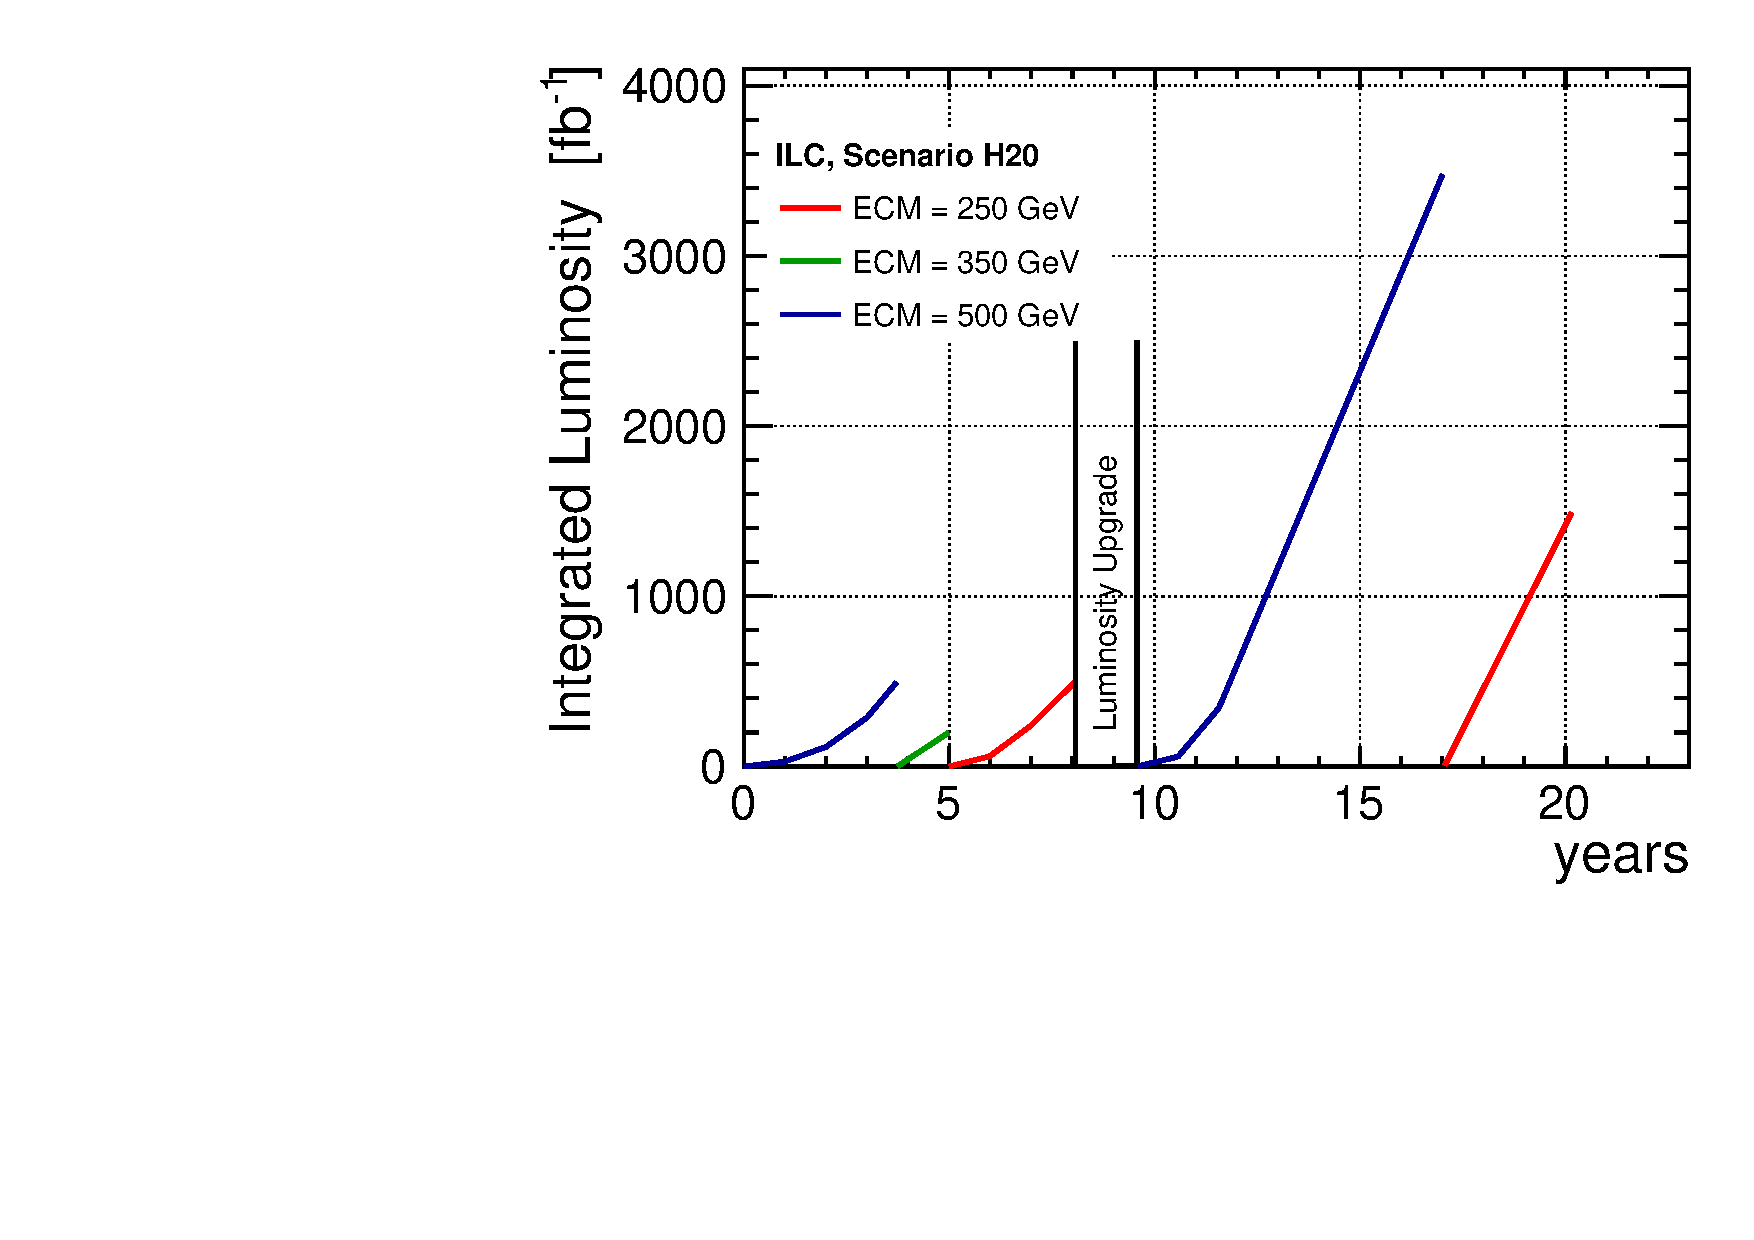
\includegraphics[width=0.85\hsize]{chapters/figures/lumi_H20.pdf}
\end{center}
\caption{The nominal 20-year running program for the 500-GeV ILC~\cite{Barklow:2015tja}.}
\label{fig:H20}
\end{figure}
%%%%%%%%%%%%%%%%%%%%%%%%%%%%%%%%%%%%%%%%%%%%%%%%%%%%%%%%%%%%%%%%%%%%%%%%%%%

After this general-purpose survey at the maximum energy, it was planned to collect dedicated datasets at lower energies, at the $t\bar{t}$ production threshold, for a precision determination of a theoretically well-defined top mass, and somewhat above the $ZH$ production threshold, near the maximum of the cross section.  The $ZH$ measurements at 250\,GeV would be a very important component of the program  even under the assumption that energies of  500\,GeV are immediately available.  This is true for two reasons.  First, in Higgsstrahlung production, each Higgs boson  is tagged by the recoil $Z$.  There are many measurements that 
rely on this tag to identify Higgs bosons or to measure absolute rates without the need to make assumptions about the Higgs decay modes.  These include the
the measurement of the normalized total cross section for the Higgsstrahlung process, the measurement  of  absolute branching ratios of the Higgs boson and the search for invisible and exotic decays.  At 500\,GeV, far above the threshold, recoil measurements become less characteristic, due to the more substantial ISR and increased amount of beamstrahlung with respect to \ 250\,GeV, and are subject to additional backgrounds.   Other measurements depend on precise reconstruction of the kinematics of the $\ee\to ZH$ process.
For example, the ultimate precision on 
the Higgs mass will be obtained using the kinematics of $Z$ recoil.  The search for deviations from the SM predictions for 
 Higgs decays requires as input a very precise value of this mass; see Sec.~\ref{sec:higgs:sigmazh}.
Another reaction that depends crucially on precise kinematic measurements is the $CP$ analysis of the $H \to \tau^+ \tau^-$ decay, discussed in Sec.~\ref{subsubsec:higgstautauCP}.

For a 500\,GeV machine running at 250\,GeV, the luminosity can be straightforwardly increased by a factor of 2 from the TDR value 
by the increase of the repetition rate for bunch trains  from 5 to 10\,Hz.  This improvement was incorporated in the plan H20 shown in Fig.~\ref{fig:H20}  even
at the initial stage of 250\,GeV running.

The H20 plan also included provision for an additional luminosity upgrade by doubling the number of bunches in each bunch 
train. This upgrade requires machine improvements as described in Sec.~\ref{subsubsec:upg-optL}, and after these improvements all further 
data would be taken in this mode.
This would give a total  4\,ab$^{-1}$ data sample at 500\,GeV.   A sample of this size is required for meaningful precisions on the top Yukawa coupling and on the Higgs self-coupling. These measurements remain by far statistically limited and  thus would profit from any further increase of the luminosity. In case of the top Yukawa coupling, it was noted that it is absolutely crucial to reach 500\,GeV, since already at 490\,GeV, thus when falling short of the target energy by only 2\%, the precision of the measurement would worsen by nearly a factor of 2. On the other hand, a moderate increase of the center-of-mass energy by 6\% to 530\,GeV would improve the precision on the top-Yukawa coupling by a factor of 2. This should be considered in the planning of the energy upgrade of an inital 250\,GeV machine, see also discussion in Sec.~\ref{subsubsec:upg-optE}.

Finally the H20 scenario planned a run at 250\,GeV, now with 4 times the TDR luminosity, to finish the collection of a 2\,ab$^{-1}$ data set.   This run would provide the ultimate precision on the Higgs boson mass and the total $ZH$ cross section. It should be stressed again that the current focus on three fixed center-of-mass energies does not preclude running at any other desired intermediate energy, \eg\ for scanning the production threshold of newly discovered particles.

At the end of this 20 year program, we envision  a further doubling of the energy to 1\,TeV.   This upgrade was presented already 
in the ILC TDR and is reviewed in Sec.~\ref{subsubsec:upg-optE}.  This energy upgrade could  possibly be preceeded by a run at the $Z$ pole if it is  required by the  physics.

%\ref{sec:design_evo}
\subsubsection{Running Scenarios for the Staged Machine}

With the introduction of the staging plan for the ILC machine construction, it was necessary to change the time ordering of the 
various energy steps in the program described in the previous subsection. However, the total integrated luminosities to be collected at each center-of-mass energy, which were already optimized for the physics goals,  were left untouched. Thus,  all physics projections based on the H20 scenario remained valid - albeit the results will arrive in a different time order. Figure~\ref{fig:H20staged-orig} shows the original plan for the time evolution of the staged H20 scenario. The assumptions differ from those listed in the previous subsection in the following points:
\begin{itemize} 
\item No 10\,Hz operation is assumed since in the 250\,GeV machine the cryomodules will be operated at full gradient and thus no spare cryo- and RF-power is available. Technically, it would be possible to increase the repetition rate (and thus the luminosity) at any time provided that resources for installing the additional cryo- and RF-power and for covering the higher operation costs could be found. This option is {\em not} included in the staging scenario.
\item The luminosity upgrade by doubling the number of bunches per train (c.f.\ Sec.~\ref{subsubsec:upg-optL}) is a smaller investment than the energy upgrade and will therefore happen first. In this plan, the second positron damping ring and the additional cryo- and RF-power needed for the luminosity doubling would  already be installed at the start of 500\,GeV operation.  Then the entire 500\,GeV run would be done at 2 times the TDR luminosity. 
\item The energy upgrade (described in\ Sec.~\ref{subsubsec:upg-optE}) requires only a relatively short machine shutdown of about one year, since major parts of the new tunnel can be constructed and the new parts of the machine can be installed without disturbing the operation of the 250-GeV machine. A shutdown is necessary only during the construction of the connections of the new parts of the  machine to the older ones.
\item After the energy upgrade the same ramp fractions as for a completely new machine are assumed, thus 10\%, 30\%, 60\% and 100\% over the first four calendar years.
\end{itemize}
With these assumptions, the real-time for realization of  the full H20 program increases from 20 to 26 years, 
mostly due to the much longer time to collect the 2\,ab$^{-1}$ at 250\,GeV without 10\,Hz operation. 


%%%%%%%%%%%%%%%%%%%%%%%%%%%%%%%%%%%%%%%%%%%%%%%%%%%%%%%%%%%%%%%%%%%%%%%%%
\begin{figure}
\begin{center}
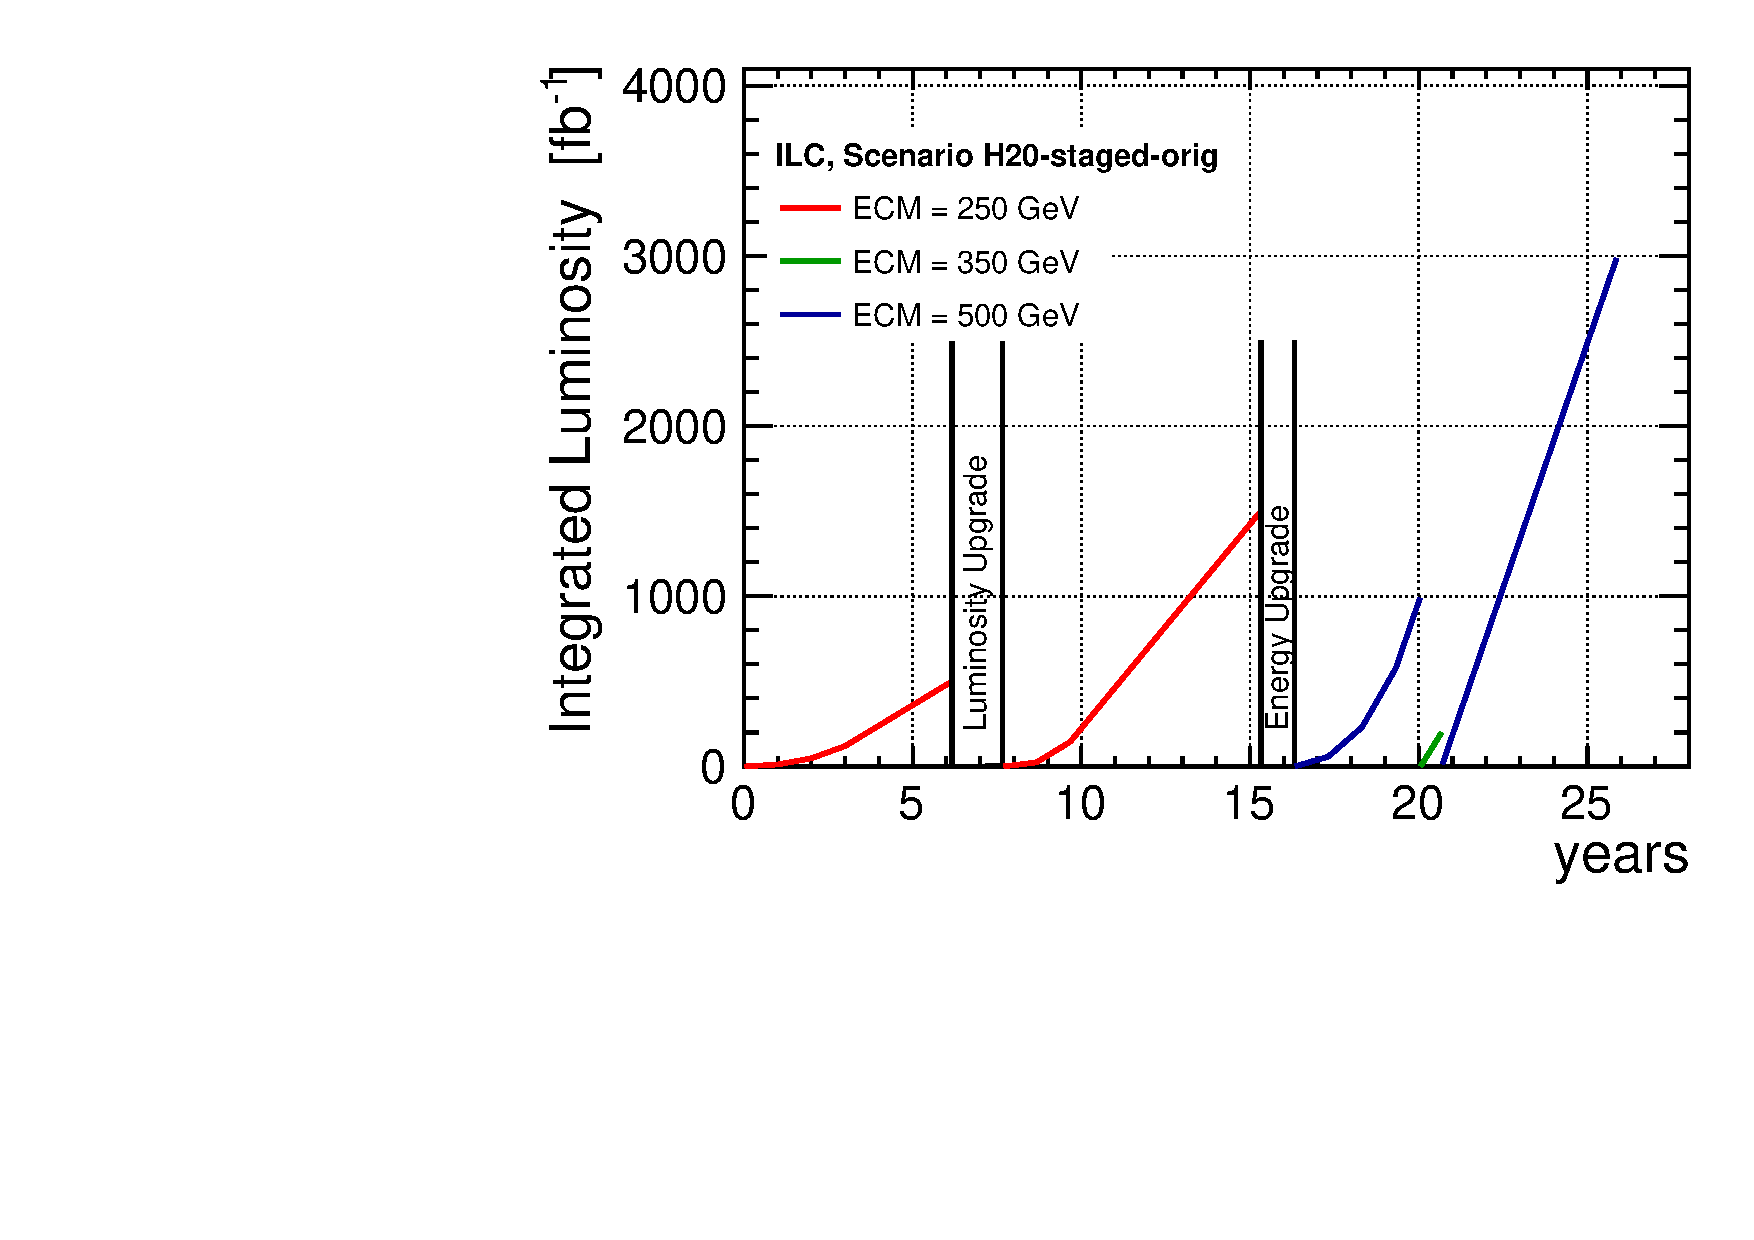
\includegraphics[width=0.85\hsize]{chapters/figures/lumi_H20-staged-orig}
\end{center}
\caption{The nominal 26-year running program for the staged ILC, starting operation at 250\,\GeV without the possibility to operate at 10\,Hz.~\cite{Fujii:2017vwa}. The integrated luminosities are the same of for the original H20 scenario.}
\label{fig:H20staged-orig}
\end{figure}
%%%%%%%%%%%%%%%%%%%%%%%%%%%%%%%%%%%%%%%%%%%%%%%%%%%%%%%%%%%%%%%%%%%%%%%%%%%

In order to mitigate the absence of the 10\,Hz operation, which would require additional investments beyond the minimal 250-GeV machine, cost neutral ways to increase the luminosity at 250\,GeV have been studied, as discussed in Sec.~\ref{sec:ilc}. In 2017, a new set of beam parameters for the 250-GeV ILC was officially adopted~\cite{bib:cr-0016}.  It is this parameter set that is shown in the column ``initial'' of Tab.~\ref{tab:ilc-params}. The 65\% increase in instantaneous luminosity w.r.t.\ the TDR parameters is achieved by reducing the horizontal emittance by a factor of 2. This leads to a larger luminosity in each bunch crossing and thus to an increase of beamstrahlung, background from $e^+e^-$ pairs and pile-up from low-$p_t$ $\gamma\gamma \to$\,hadrons events. Neither these effects, nor the slightly wider luminosity spectrum which results from the increased beamstrahlung are included in the physics case studies presented in the following sections, since no new Monte-Carlo samples could be produced (and analysed) since the new beam parameters became available. However, even with the new beam parameters the background conditions at 250\,GeV do not become worse than what is expected at 500\,GeV, a case already studied in detail.  The ILC detectors have actually been designed for high performance in the more difficult  beam conditions at 1\,TeV. Therefore, the impact of the new beam parameters on the majority of the physics anayses is expected to be minor. The analysis most strongly affected is the mass measurement of the Higgs boson via the leptonic recoil method, described in Sec.~\ref{sec:higgs:sigmazh}. For this analysis, the new beam parameters have been estimated to result in a relative degradation of the ultimate precision on the Higgs mass by about 25\%~\cite{bib:jeans_awlc17} compared to the same amount of total luminosity collected with the TDR beam parameters.  This still corresponds to an impressive 
Higgs mass measurement to better than 20\,MeV. 

We have already shown in Fig.~\ref{fig:H20staged} the default running scenario for the staged ILC based on the new beam parameters for 250\,GeV~\cite{bib:cr-0016}. Compared to Fig.~\ref{fig:H20staged-orig}, the total run time shortens from 26 years to 22 years, thus recovering about 2/3 of the original increase in running time. A full-scale Monte-Carlo production with the new beam parameters and based on the ILD detector concept is planned for 2019.


None of the running scenarios explicitly includes the option to increase the positron polarisation to 60\% when operating at a center-of-mass energy of 500\,GeV. Numerous studies~\cite{Fujii:2018mli, Habermehl:417605, Moortgat-Picka:2015yla, Aurand:2009kp, MoortgatPick:2005cw} have shown that all physics measurements will profit from the corresponding increases in effective luminosity and effective polarisation. In this respect, all physics projections for 500\,GeV are still quite conservative.
